\subsection{Shape Matching}
\label{subsec:Shape Matching}


Here, we give shape matching a more extensive definition: finding the correspondence(point-wise, pair-wise) between two rigid or non-rigid deformable geometric data sets.

\subsubsection{Rigid registration}
\label{subsubsec:Rigid registration}

Rigid registration is a fundamental task in computer graphics and geometry processing.
It aims at finding a suitable set of corresponding points on source and target point set.
The $Iterative~Closest~Point$(ICP) addresses this problem by assuming the input data to be in coarse alignment.
Under this assumption, a set of correspondences can be obtained by querying closest points on the target geometry.
Given two surfaces $\mathcal{X}$, $\mathcal{Y}$, it is formulated as

\small{
\begin{equation}
 \label{eq:ICP}
 \mathop{\argmin}_{R,t}\int_{\mathcal{X}}^{}\varphi(R\mathbf{x}+t,\mathcal{Y})d\mathbf{x}+I_{\mathcal{SO}(k)}(R)
\end{equation}
}
\\
where $R$ is a rotation matrix,
$t$ is a translation vector,
$\mathbf{x}$ is a point on the source geometry.
The quality of a registration is evaluated by the metric $\varphi(\mathbf{x},\mathbf{y})=\|\mathbf{x}-\mathbf{y}\|{_2^2}$, i.e., classical ICP is in a least-square sense which would fail with outliers.

Now that sparse regularization methods excels in processing data set with noises or outliers,
\cite{bouaziz2013sparse} tries to formulate the local alignment problem as recovering rigid transformation that minimizes the number of zero distances between two correspondences.
Since \cite{chartrand2007exact} shows that $\ell_{p}$ norms with $p<1$ outperform the $l_1$ norm in inducing sparsity and \cite{elad2010sparse} also illustrates the tendency of $\ell_{p}$($0<p<1$)norms to drive results to become sparse.
\cite{bouaziz2013sparse} adopts $l_{p}$($0\le p\le1$) norm based sparse regularizer to obtain an heuristic-free, robust rigid registration algorithm by modifying

\small{
\begin{equation}
 \label{eq:permutedsparse}
 \varphi(\mathbf{x},\mathbf{y})=\|\mathbf{x}-\mathbf{y}\|{_2^{p}}
\end{equation}
}

Figure~\ref{fig:sparseICP}is the registration results of sparse ICP under different values of $p$ among which it can be found that $0<p<1$ reduces better results,
but the value of $p$ is selected according to the experiments to offer a trade-off between performance and robustness which may make the sparse ICP unpractical.

\begin{figure}[ht]
  \centering
  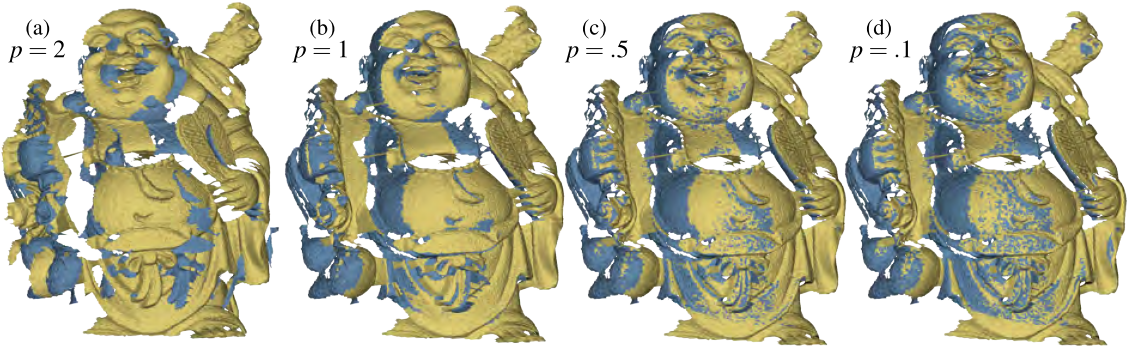
\includegraphics[width=3in]{images/sparseICP}
  \caption{Sparse regularization: rigid registration results using sparse ICP\cite{chartrand2007exact} under different $l_{p}$ norms.}
  \label{fig:sparseICP}
\end{figure}

\subsubsection{Non-rigid shape matching}
\label{subsubsec:non-rigid shape matching}

Matching of deformable shapes is a notoriously difficult problem playing an important role in many application, non-rigid matching typically uses point-wise representation of correspondence, which results in the number of degrees of freedom growing exponentially with the number of matched points.

Recently, \cite{ovsjanikov2012functional} introduces a functional representation for correspondences which are modeled as the correspondences between functions on two shapes rather than points.
Mathematically, let $X$ and $Y$ be two shapes equipped with bases $\{\phi_{i}\}_{i\ge1}$ and $\{\psi_{j}\}_{j\ge1}$ respectively,
any real function $f: X\to \mathbb{R}$ and $g=T(f): Y\to \mathbb{R}$ can be represented as $f=\sum_{i\ge1}^{}a_{i}\phi_{i}$ and $g=\sum_{j\ge1}^{}b_{j}\psi_{j}$.
Taking discretized functions $\phi_{i}$ and $\psi_{j}$ as the columns of bases matrices $\Phi$ and $\Psi$,
the function vectors can be represented as
$\mathbf{f}=\Phi \mathbf{a}$ and
$\mathbf{g}=\Psi \mathbf{b}$, and then from
$\Psi \mathbf{b}=T(\Phi \mathbf{a})=\Psi C^{T}\mathbf{a}$,
the relationship between two coefficients is clear that $\mathbf{b^{T}}=\mathbf{a^{T}}C$.
Thus, the matrix $C$ fully encodes the linear map $T$ between the functional spaces.


In case the shapes $X$ and $Y$ are isometric and the corresponding Laplace-Beltrami operators have simple spectra,
the harmonic bases(Laplacian eigenfunctions) have a compatible behavior, $\psi_{i}=T(\phi_{i})$ such that $c_{ij}=\delta_{ij}$.
Choosing the discretized eigenfunctions of the Laplace-Beltrami operator as $\Phi$ and $\Psi$ causes every low-distortion correspondence being represented by a nearly diagonal, and therefore very sparse matrix $C$.

Based on the above theory, \cite{pokrass2013sparse} firstly gets two collections of similar functions $\{f_{i}:X\to \mathbb{R}\}$ and $\{g_{j}:Y\to \mathbb{R}\}$ using some region detection process like\cite{litman2011diffusion}. \parpic[r]{\label{fig:regionmatching}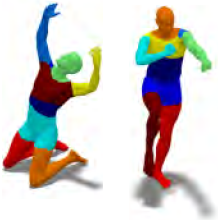
\includegraphics[width=0.4\linewidth]{images/matching_function}}As shown in the right figure, different colors represent different functions and the correspondence of these two collections of functions is unknown, i.e., we do not know to which $g_{j}$ in $Y$ a $f_{i}$ in $X$ corresponds.
\cite{pokrass2013sparse} adopts an unknown permutation matrix $\mathbf{\Pi}$ to express this ordering. Finally, the robust permuted sparse coding is formulated as following

\small{
\begin{equation}
 \label{eq:non-rigid shape matching}
 \min_{C,O,\Pi}\frac{1}{2} \|\Pi B - AC - O \|{_{F}^2} + \lambda\| W \odot C\|_1+\mu\|O\|_{2,1}
\end{equation}
}
\\
where $W$ is assigned with larger weights in off-diagonal part and small weights in diagonal part to promote diagonal solutions, $\|O\|_{2,1}$ promotes row-wise sparsity allowing to absorb the errors in the data term corresponding to the rows of $A$ having no corresponding rows in $B$.
Figure~\ref{fig:non-rigid matching} shows the correspondences between non-isometric shapes. This method relies on the region detection technique and assumption: near-isometric shapes.

\begin{figure}[ht]
  \centering
  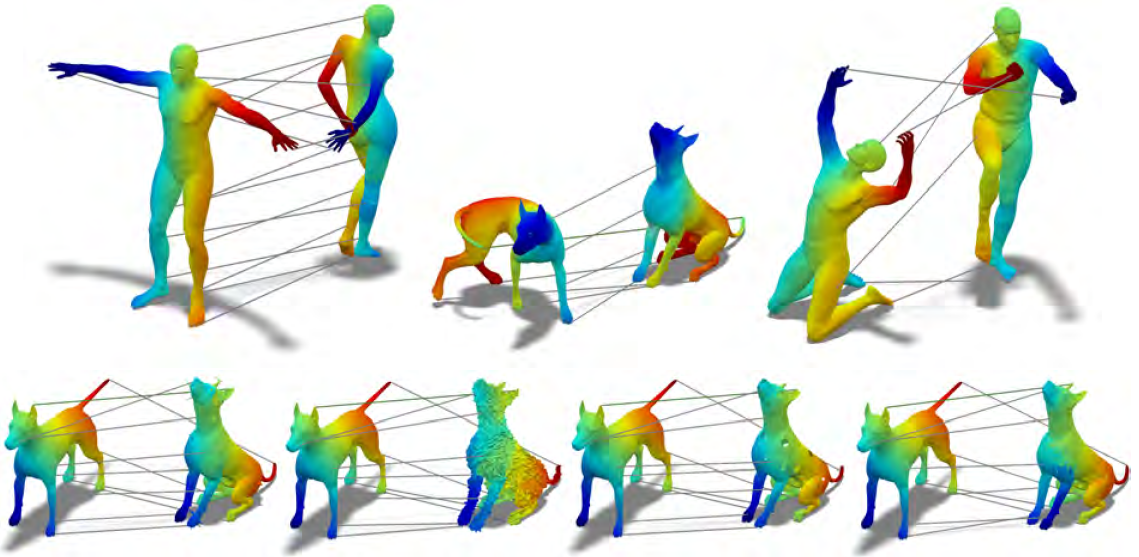
\includegraphics[width=3in]{images/matching_L1}
  \caption{Sparse regularization: non-rigid shape matching \cite{wang2014decoupling}. First row: point-to-point correspondences between different non-isometric shapes. Second row: point-to-point correspondence between SHREC shapes undergoing nearly isometric deformations and noise.}
  \label{fig:non-rigid matching}
\end{figure}


\subsubsection{Co-segmentation}
\label{subsubsec:co-segmentation}

Co-segmentation aims to consistently segment a group of shapes and obtain the correspondence between resulted segments simultaneously. As the right figure in Figure~\ref{fig:co-segmentation}shows, corresponding parts are labeled in the same colors.
To be more intuitive and efficient, \cite{hu2012co} processes co-segmentation on patch-level instead of face-level like many other works.

So they firstly over-segment all the models(left in Figure~\ref{fig:co-segmentation}) followed by calculating their feature vectors using some feature descriptors.
For example, Figure~\ref{fig:co-segmentationAGD} shows the colormaps of average geodesic distance(AGD) features of two tables with over-segmented patches, and actually there are $H=5$ feature descriptors.
They define the feature vector as a histogram of the feature measurement on the triangles of that patch.
Then it is obvious that two corresponding patches have similar distributions, which means their feature vectors lie in a common subspace generated by standard basis corresponding to these nonzero entries.
Based on this observation, they regard co-segmentation as a subspace clustering problem since the final segments are all clustering of patches.

\begin{figure}[ht]
  \centering
  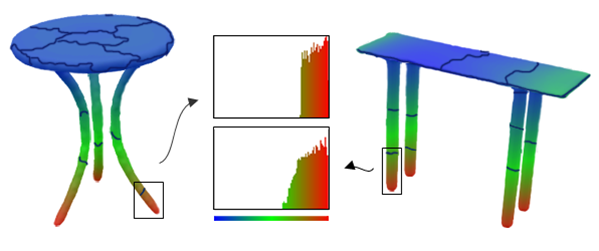
\includegraphics[width=3in]{images/co-segmentationAGD}
  \caption{Sparse regularization: co-segmentation\cite{hu2012co}. Colormaps of AGD features of two tables with over-segmented patches. The AGD feature vectors of the two patches(marked in rectangles) from each table's leg have similar distribution, as shown in histograms in the middle. It can be seen that these two feature vectors lie in the common subspace generated by standard basis corresponding to the nonzero entries.}
  \label{fig:co-segmentationAGD}
\end{figure}


Since that each data point(here is the feature vector) in a union of linear subspaces can always be represented as a linear combination of the points belonging to the same linear subspace
and thus the combination could be sparse if the point is written as a linear combination of all other points. Following\cite{elhamifar2009sparse,wang2011efficient}, finding the sparse combination matrix for the single-feature co-segmentation is formulated as

\small{
\begin{equation}
 \label{eq:SSC}
 \begin{split}
 &\min_{W_{h}}\|X_{h}W_{h}-X_{h}\|{_{F}^2}+\lambda\|W_{h}^{T}W_{h}\|_{1,1} \\
 &\mathrm{s.t.}~W_{h}\ge0,~\textrm{diag}(W_{h})=0
 \end{split}
\end{equation}
}
\\
where $h$ corresponds to the $h$-th feature descriptor,
the feature matrix $X_{h}=[x_{h1},x_{h2},\cdots,x_{hN}]$ is constructed with $x_{hi}$ which is the feature vector of the $i$-th patch($i=1,2,\cdots,N$).
$\|W_{h}^{T}W_{h}\|_{1,1}$ is seen as a penalty item in the optimization, which favors the sparsity of the optimal solution $\overline{W_{h}}$ of which each entry measures the linear correlation between two points in the meshes.
After defining the affinity matrix $S=(s_{ij})$ as $s_{ij}=|\overline{w_{h}}_{ij}|+|\overline{w_{h}}_{ji}|$, the NCut method\cite{shi2000normalized} is applied to get the co-segmentation results.

However, single one feature is not enough for co-segmenting different categories of models.
Taking two following things into account:
finding the most similar patch pairs considering selected features and corresponding patches need not be similar in these features,
\cite{hu2012co} adds the consistent multi-feature penalty to ensure the co-segmentation results consistent with different feature spaces by combing $H$ feature descriptors

\small{
\begin{equation}
 \label{eq:coseg1}
 \begin{split}
 &\min_{W_{1},\cdots,W_{H}}\sum_{h=1}^{H}\mathcal{F}(W_{h})+\mathcal{P}_{cons}(W_1,W_2,\cdots,W_H)\\
 &\mathrm{s.t.}~W_{h}\ge0,~\textrm{diag}(W_{h})=0,h=1,2,\cdots,H.
 \end{split}
\end{equation}
}
\\
where $\mathcal{P}_{cons}$ is the penalty on the matrices $W_1,W_2,\cdots,W_H$

\small{
\begin{equation}
 \label{eq:coseg2}
 \mathcal{P}_{cons}(W_1,W_2,\cdots,W_H)=\alpha\|W\|_{2,1}+\beta\|W\|_{1,1}\\
\end{equation}
}
\\
here the $H\times N^2$ matrix $W$ is formed by concatenating $W_1,W_2,\cdots,W_H$(each matrix in one row) together:

\small{
\begin{equation}
 \label{eq:coseg3}
 W = {\left[ \begin{array}{cccc}
 (W_1)_{11} & (W_1)_{12} & \cdots & (W_1)_{N^2}\\
 (W_2)_{11} & (W_2)_{12} & \cdots & (W_2)_{N^2}\\
 \vdots & \vdots & \ddots & \vdots\\
 (W_{H})_{11} & (W_{H})_{12} & \cdots & (W_{H})_{N^2}
 \end{array}
 \right]}
\end{equation}
}
\\
the $\ell_{2,1}$ penalty on $W$ induces column sparsity of $W$ such that most columns of $W$ are shrunken to be entirely zero, which means that the corresponding pairs of patches will likely not be in the same cluster.
The $\ell_{1,1}$ penalty on $W$ induces the sparsity within each column of $W$.
This means that for each non-zero column, that is for each similar patch pair, only a subset of features are actually used to measure their similarity.
Hence this term enables the prominent features to pop up and guarantees the sparsity-consistency of the matrices $W_1,W_2,\cdots,W_H$.

Notice that without $\mathcal{P}_{cons}$, the formulation~(\ref{eq:coseg1}) will reduce to a naive solution which is exactly the same as applying subspace clustering to each feature matrix $X_{h}$ independently.

\begin{figure}[ht]
  \centering
  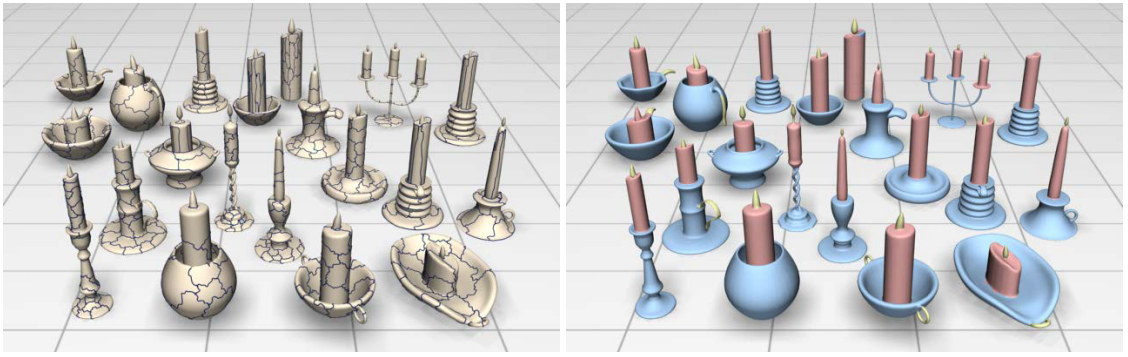
\includegraphics[width=3in]{images/co-segmentation}
  \caption{Sparse regularization: co-segmentation\cite{hu2012co}. Left shows the over segmented patches that will be clustered to get the co-segmentation result.}
  \label{fig:co-segmentation}
\end{figure}

